
\documentclass[aspectratio=169]{beamer}
\usetheme{Madrid}
\usecolortheme{seahorse} % slightly more modern color
\usepackage{amsmath, amssymb, booktabs, bm, multirow}
\usepackage{graphicx}
\usepackage{ctex}
\usepackage{xcolor}
\usepackage{hyperref}
\hypersetup{
    colorlinks=true,      % Enable colored links
    linkcolor=blue!70!black, % Consistent with highlight color
    urlcolor=red!70!black,   % Slightly less aggressive red
    citecolor=green!65!black, % Softer green for readability
    linkbordercolor={0 0 0}   % No border color (rarely used)
}

\usepackage[ruled,vlined,linesnumbered]{algorithm2e}
\usepackage{listings}
\lstset{
    language=Python,
    basicstyle=\ttfamily\scriptsize,  % beamer中用scriptsize
    keywordstyle=\color{blue},
    commentstyle=\color{green!50!black},
    stringstyle=\color{red},
    numbers=left,
    numberstyle=\tiny\color{gray},
    breaklines=true,
    showstringspaces=false,
    frame=shadowbox,  % beamer中更美观
    backgroundcolor=\color{gray!5}
}


% ---------------------------------------------------------------------------
% 排版与版式：统一间距与列表样式，避免拥挤
% ---------------------------------------------------------------------------
\setbeamertemplate{footline}[frame number]
\AtBeginSection[]{
  \begin{frame}{目录}
    \tableofcontents[currentsection, hideothersubsections]
  \end{frame}
}
\setlength{\leftmargini}{1.2em}
\setlength{\itemsep}{0.4em}
\setlength{\parskip}{0.35em}
\setbeamertemplate{itemize item}{\scriptsize\raise0.5pt\hbox{$\bullet$}}


% Graphics path for including figures
\graphicspath{{./}{figures/}}

% Metadata
\title{Reinforcement Learning for LLM}
\author{\href{https://b23.tv/a0Bb9Z1}{Bilibili 以往的月}}
\institute{\href{https://maosong.website/}{Homepage}}
\date{\today}

\begin{document}

\frame{\titlepage}

\begin{frame}{目录}
  \tableofcontents
\end{frame}

% ===========================================================================
\section{Introduction}
% ===========================================================================

\begin{frame}{The Goal of This Tutorial}

  \begin{block}{The Goal of This Tutorial}
      （建模）LLM如何与RL对应？（算法）GRPO, PPO, DPO 背后的原理是什么？（实验）如何实现？
  \end{block}

  \begin{figure}
    \centering
    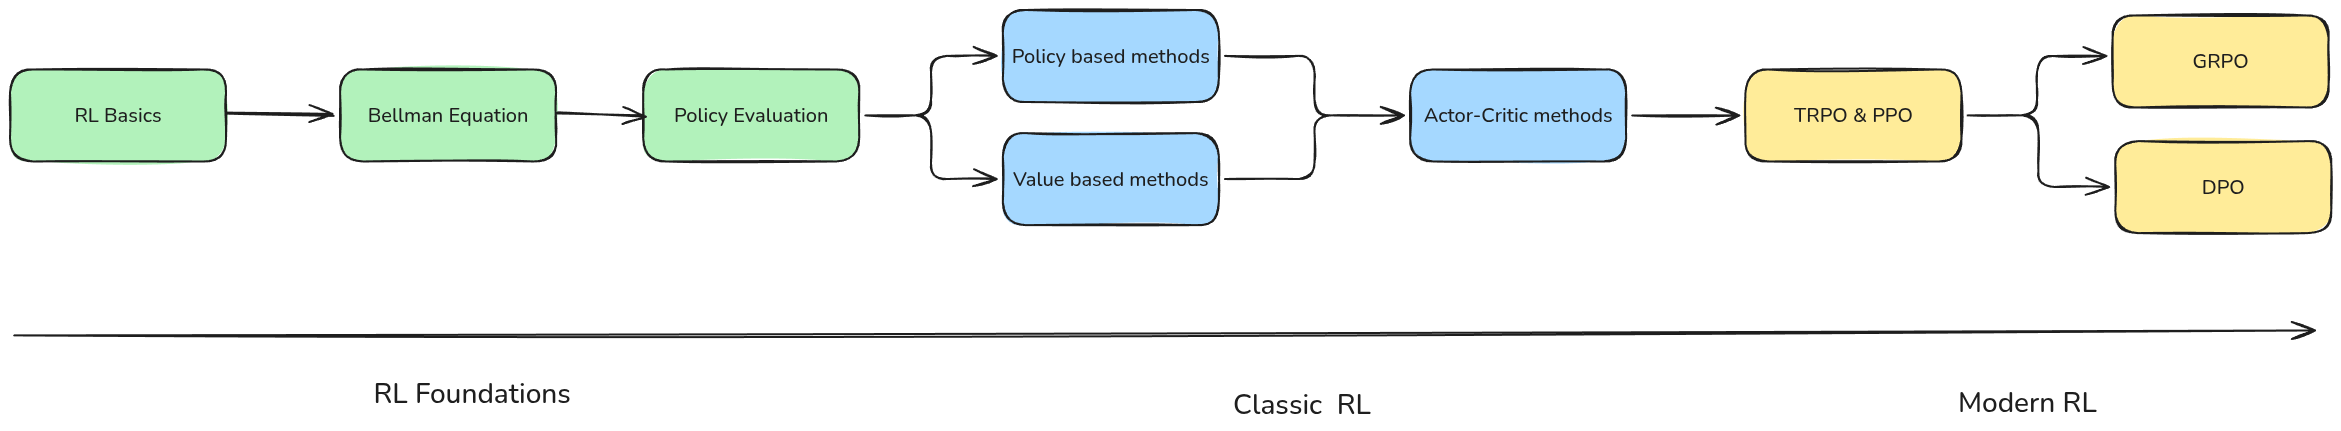
\includegraphics[width=0.9\linewidth]{../images/RL-LLM-pipeline.png}
    \caption{Pipeline of this RL-LLM tutorial series}
    \label{fig:rl_llm_pipeline}
  \end{figure}

  \begin{block}{References}
    \begin{itemize}
        \item \href{https://ernestryu.com/courses/RL-LLM.html}{Reinforcement Learning for Large Language Models}
        \item \href{https://shiyuzhao.westlake.edu.cn/info/1042/1852.htm}{强化学习的数学原理}
    \end{itemize}
  \end{block}

\end{frame}

\section{Reinforcement Learning: Basics}

\begin{frame}{What is Reinforcement Learning?}
    \begin{block}{Core Idea}
        RL的基本思想是：让agent通过与环境交互，学习到最优策略。
    \end{block}
    \vspace{-0.3cm}
    \begin{figure}
        \centering
        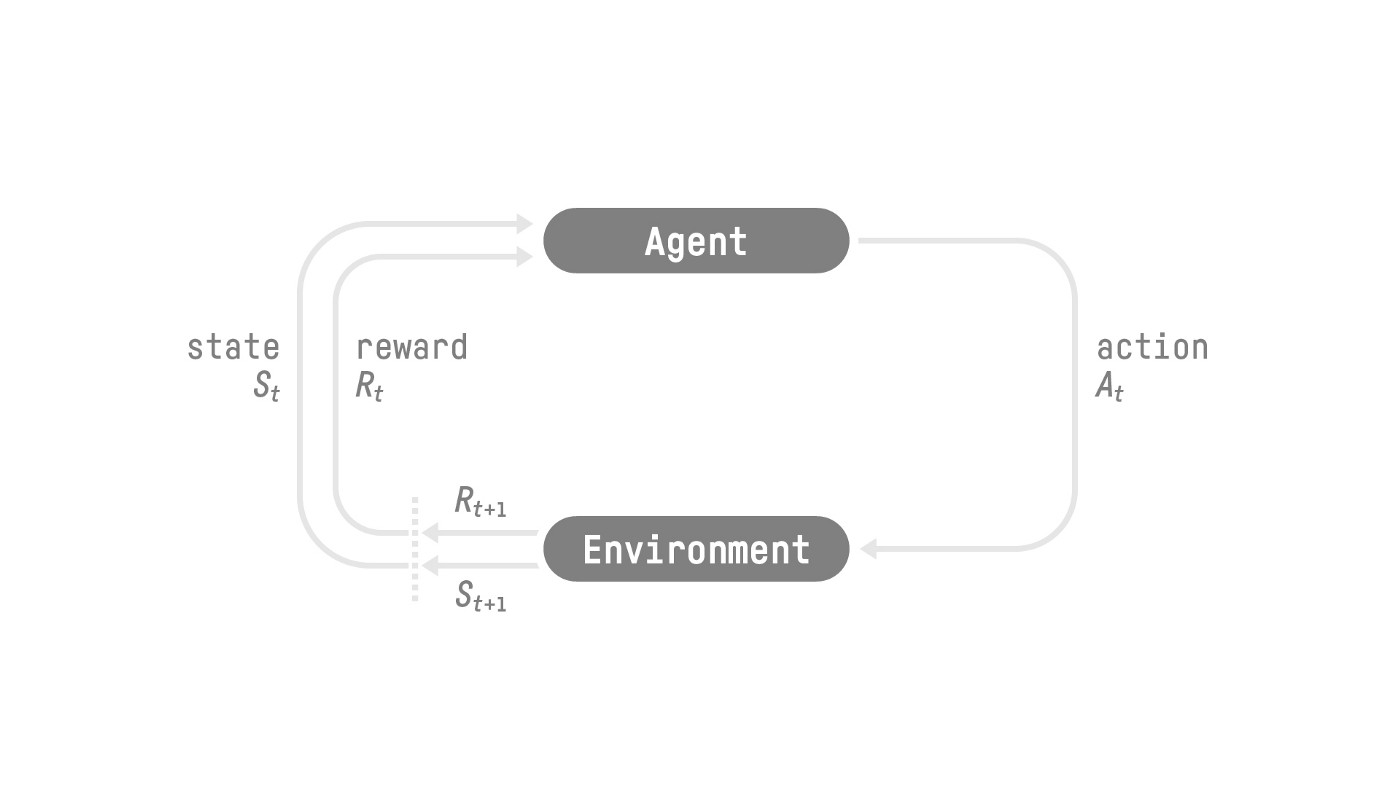
\includegraphics[width=0.5\linewidth]{../images/RL-process.png}
        \vspace{-0.5cm}
        \caption{Illustration of the RL process}
        \label{fig:rl_process}
    \end{figure}
    \vspace{-0.3cm}
    \begin{definition}[Reinforcement Learning]
        强化学习是一个通过构建可以与环境进行交互的 agent 来解决控制和决策任务的学习框架，交互的方式为 agent 执行 action, 然后环境给予奖励
    \end{definition}
\end{frame}

\begin{frame}{Markov Decision Process (MDP)}
    \begin{definition}{Markov Decision Process (MDP)}
        马尔可夫决策过程（Markov Decision Process, MDP）是描述强化学习环境的数学模型，形式化为：
    
        \begin{itemize}
            \item \textbf{状态 (State)}: $s_t \in \mathcal{S}$, $\mathcal{S}$ 为状态空间。
            \item \textbf{动作 (Action)}: $a_t \in \mathcal{A}, \mathcal{A}$ 为动作空间。
            \item \textbf{奖励 (Reward)}: $r_t \in \mathbb{R}$，环境对 agent 执行动作 $a_t$ 的反馈。
            \item \textbf{终止时间}: $T$，且定义 $s_T = \langle\text{term}\rangle$ 为终止状态。
            \item \textbf{初始状态分布}: $s_0 \sim p_0$.
            \item \textbf{状态转移概率 (Transition Probability)}: $(r_t, s_{t+1}) \sim p(\cdot, \cdot \mid s_t, a_t)$.
            \item \textbf{马尔可夫性 (Markov Property)}: \\
                \begin{equation}
                    p(s_{t+1} \mid s_t, a_t, \ldots) = p(s_{t+1} \mid s_t, a_t),\ p(r_t \mid s_t, a_t, \ldots) = p(r_t \mid s_t, a_t)
                \end{equation}
        \end{itemize}
    \end{definition}
\end{frame}


\begin{frame}{Trajectory}
    \textbf{轨迹（Trajectory）：} $\tau=(s_0, a_0, r_0, s_1, a_1, r_1, \ldots, s_{T-1}, a_{T-1}, r_{T-1}, s_T)$.

    我们可以将轨迹写为如下形式

    \begin{equation}
        p(\tau\mid s_0, \pi, p) =  p_0(s_0)\prod_{i=1}^{T-1}\pi(a_t\mid s_t)p(r_t, s_{t+1}\mid r_t,s_t)
    \end{equation}

    可以看到，轨迹的概率分布是由初始状态分布，策略，以及环境模型共同决定的，我们可以将其记为 $\tau\sim(p_0,\pi, p)$.
    \begin{block}{Remark}
        \begin{itemize}
            \item 轨迹的概率分布是由初始状态分布，策略，以及环境模型共同决定的，我们可以将其记为 $\tau\sim(p_0,\pi, p)$.
            \item 我们在这个tutorial中仅考虑有限horizon的MDP, 即 $T<\infty$.
        \end{itemize}
    \end{block}
\end{frame}

\begin{frame}{Expected Return}
    \begin{definition}[Expected Return]
        \begin{equation}
            R(\tau) = \sum_{t=0}^{T-1} \gamma^t r_t
        \end{equation}
        其中 $\gamma\in(0,1)$ 是 discount factor, 用于将未来的奖励折现到当前时刻。
    \end{definition}

    一般我们会将 expected return 记为 $G_0$, 即
    \begin{equation}
        G_0 = \sum_{t=0}^{T-1} \gamma^t r_t
    \end{equation}

    $G_0$ 存在如下递推关系
    \begin{equation}
        G_0 = r_0 + \gamma G_1
    \end{equation}
    \footnotetext{后续我们将会交错使用 $G_0$ 和 $R(\tau)$ 来表示 expected return.}
\end{frame}

\begin{frame}{Objective of RL}
    \begin{block}{Reward Hypothesis}
        所有的目标都可以被描述为最大化 expected return.
    \end{block}

    \begin{block}{Objective}
        RL的最终目标为最大化 expected return. 形式化为
        \begin{equation}
            \max_{\pi}\quad \mathbb{E}_{\tau\sim(p_0,\pi, p)}^\pi R(\tau)
        \end{equation}
    \end{block}
\end{frame}

\begin{frame}{Connection with LLM}
    LLM 的建模方式：
    \begin{equation}
        y_i \sim \mathrm{LLM}(\cdot\mid y_{<i}, x)
    \end{equation}
    其中 $x$ 是输入的prompt, $y_{<i}$ 是已经生成的部分，$y_i$ 是下一个要生成的token.

    \begin{table}[h!]
        \centering
        \begin{tabular}{ccc}
            \toprule
            \textbf{RL} & \textbf{LLM} & \textbf{Explanation}\\
            \midrule
            policy $\pi$        & LLM $\mathrm{LLM}(\cdot\mid y_{<i}, x)$ & - \\
            initial state $s_0$ & prompt $x$            & - \\
            action $a_t$        & current token $y_i$   & action space: the vocabulary of the LLM \\
            state $s_t$         & context $(y_{<i}, x)$ & state space: the context of the LLM, huge \\
            \bottomrule
        \end{tabular}
    \end{table}

    \begin{block}{Remark}
        注意到我们并没有对 environment 和 reward 进行建模，我们可以这样进行理解:

        \begin{enumerate}
            \item LLM 中的 environment 仅仅是对 token 进行简单拼接, $s_{t+1} = \mathrm{concate}(y_i, s_t)$.
            \item reward 由 verifier, reward model (PRM, ORM) 或者 human feedback 给定
        \end{enumerate}
    \end{block}
\end{frame}

\begin{frame}{Takeaway}
    \begin{itemize}
        \item RL的基础是MDP, 其核心假设是markov property, 即未来的状态和奖励只与当前状态和动作有关，与历史状态和动作无关。
        \item RL通过reward hypothesis, 将目标转化为最大化expected return.
        \item 从RL角度来看，LLM 本身是一个policy, 其初始状态为 prompt, 动作空间为 vocabulary 中的 token index, 奖励由多方面给定，environment 仅仅是对 token 进行简单拼接。

    \end{itemize}
\end{frame}


\section{Reinforcement Learning: Bellman Equation}

\begin{frame}{Why Bellman Equation?}
    \begin{block}{Motivation}
        在强化学习中，我们关心的不是某一步立即得到的 reward，
        而是 agent 从当前状态出发，在未来持续决策后能够获得的累计回报。
    \end{block}
    \begin{block}{Difficulty}
        但是，累计回报依赖于整条未来轨迹：
        后续会到达什么状态、采取什么动作、获得什么奖励，都是随机的。
        因此直接分析 expected return 往往比较困难。
    \end{block}
    \begin{block}{Core Idea}
        \textbf{将长期回报写成“当前一步的收益 + 下一状态的未来价值”}，从而把一个全局问题转化为递推问题。
        \begin{equation}
            \text{long-term value} = \text{immediate reward} + \text{discounted future value}
        \end{equation}
    \end{block}
\end{frame}

\begin{frame}{Value function and Q function}
\begin{definition}[Value function]
    Value function 定义为：
        \begin{equation}
            V^{\pi}(s) = \mathbb{E}^{\pi}[G_0\mid s_0=s]
        \end{equation}
        value function 的具体含义为：\textbf{agent 从当前状态 $s$ 出发，一直遵循当前策略 $\pi$， 最后获取到的 expected return}.
\end{definition}

\begin{definition}[Q function]
    Q function 定义为：
    \begin{equation}
        Q^{\pi}(s,a) = \mathbb{E}^{\pi}[G_0\mid s_0=s, a_0=a]
    \end{equation}
    Q function 的具体含义为：\textbf{agent 从当前状态 $s$ 出发，执行动作 $a$, 一直遵循当前策略 $\pi$, 最后获取到的 expected return}.
\end{definition}

\footnotetext{在不影响理解的情况下，我们省略 $\tau\sim (p_0,\pi, p)$ 的标记}
\end{frame}

\begin{frame}{Relationship between value function and Q function}
    \begin{block}{Relationship between value function and Q function}
        Value function 和 Q function 之间存在如下关系：
        \begin{equation}
            V^{\pi}(s)  = \mathbb{E}_{a_0\sim \pi(\cdot\mid s_0)}[Q^{\pi}(s,a)]
        \end{equation}
        即 value function 是 Q function 的期望。
    \end{block}
    \begin{proof}
        由全概率公式，我们有
        \begin{equation}
            \mathbb{E}[G_0\mid s_0=s] = \sum_{a\in\mathcal{A}}\mathbb{E}\left[G_0\mid s_t=s, a_0=a\right]\pi(a\mid s_0=s)
        \end{equation}
        即
        \begin{equation}
            \boxed{V^{\pi}(s)  = \mathbb{E}_{a_0\sim \pi(\cdot\mid s_0)}[Q^{\pi}(s,a)]}
        \end{equation}
    \end{proof}
\end{frame}

\begin{frame}{Iterative property}
    Value function 和 Q function 存在如下递推关系
    \begin{align}
        V^\pi(s) &= \mathbb{E}_{a\sim \pi(\cdot\mid s),\ (r,s')\sim p(\cdot,\cdot\mid s,a)}[r + \gamma V^\pi(s')\mid s]\\
        Q^\pi(s,a) &= \mathbb{E}_{(r,s')\sim p(\cdot,\cdot\mid s,a),\ a'\sim \pi(\cdot\mid s')}[r + \gamma Q^\pi(s',a')\mid s,a]
    \end{align}
    \begin{proof}
        \begin{align}
            V^{\pi}(s) &= \mathbb{E}^{\pi}[r_0+\gamma G_1\mid s_0=s]\\
            &= \mathbb{E}_{a\sim \pi(\cdot\mid s),\ (r,s')\sim p(\cdot,\cdot\mid s,a)}\left[\mathbb{E}^\pi[r + \gamma G_1\mid s,a,r,s']\mid s\right]\\
            &\overset{\text{Markov}}{=} \mathbb{E}_{a\sim \pi(\cdot\mid s),\ (r,s')\sim p(\cdot,\cdot\mid s,a)}\left[r + \gamma \mathbb{E}^\pi[G_1\mid s',a']\mid s\right]\\
            &= \mathbb{E}_{a\sim \pi(\cdot\mid s),\ (r,s')\sim p(\cdot,\cdot\mid s,a)}\left[r + \gamma V^\pi[s')\mid s\right]
        \end{align}
    \end{proof}
\end{frame}


\begin{frame}{Bellman Equation (Value function)}
    \begin{theorem}[Bellman Equation]
        令 $\pi$ 为一个策略，假设 $\gamma\in(0,1)$, $|\mathcal{S}|<\infty$ 以及 $|r|\leq R<\infty, \mathrm{a.s.}$. 
        那么 $\pi$ 对应的 value function $V^\pi:\mathcal{S}^+\to\mathbb{R}$ 存在，且满足 Bellman equation:
        \begin{equation}
        V^\pi(s) = \mathbb{E}_{a\sim \pi(\cdot\mid s),\ (r,s')\sim p(\cdot,\cdot\mid s,a_0))}\left[r+\gamma V(s')\mid s\right]
        \end{equation}
        反之，如果存在函数 $V:\mathcal{S}^+\to\mathbb{R}$ 满足 Bellman equation, 则 $V=V^\pi$.
    \end{theorem}
\end{frame}

\begin{frame}{Fixed Point Theorem*}
    \begin{definition}[Fix Point]
        对于函数 $f:\mathbb{R}^n\to\mathbb{R}^n$, 如果一个点 $x^*\in\mathbb{R}^n$ 满足
        \begin{equation}
        f(x^*)=x^*
        \end{equation}
        则我们称 $x^*$ 是函数 $f$ 的 \textbf{fixed point}.
    \end{definition}

    \begin{definition}[Contraction mapping]
        对于函数 $f:\mathbb{R}^n\to\mathbb{R}^n$, 如果存在 $\gamma\in(0,1)$ 满足
        \begin{equation}
            \|f(x_1)-f(x_2)\| \leq \gamma \|x_1-x_2\|,\forall\ x_1,x_2\in\mathbb{R}^n
        \end{equation}
        则我们称 $f$ 是一个 \textbf{contraction mapping}. 这里 $\|\cdot\|$ 是一个 matrix norm.
    \end{definition}
\end{frame}


\begin{frame}{Fixed Point Theorem*}
    \begin{theorem}[Fixed Point Theorem]
        给定函数 $f:\mathbb{R}^n\to\mathbb{R}^n$, 如果 $f$ 是一个 contraction mapping, 则 $f$ 具有如下性质
        \begin{enumerate}
            \item Existence: 存在 fixed point $x^*\in\mathbb{R}^n$ 满足 $f(x^*)=x^*$.
            \item Uniqueness: fixed point $x^*$ 唯一。
            \item Algorithm: 对任意 $x_0\in\mathbb{R}^n$, 使用迭代算法 $x_{k+1}=f(x_k)$ 产生的序列 $\{x_k\}_{k=1}^{\infty}$ 收敛到 fixed point $x*$, 且收敛速度为指数级。
        \end{enumerate}
    \end{theorem}
    \begin{proof}
        证明见附录 Frame~\ref{fixed-point-theorem}
    \end{proof}
\end{frame}


\begin{frame}{Bellman Equation Theorem--Proof}
    \begin{proof}
    由 $V^\pi$ 定义，我们有
    \begin{equation}
        \left|\sum_{t=0}^{\infty}\gamma^tr_t\right|\leq \sum_{t=0}^\infty \gamma^t R=\frac{R}{1-\gamma}<\infty
    \end{equation}
    因此，$\sum_{t=0}^{\infty}\gamma^tr_t$ 是一个绝对收敛的序列，从而其期望存在且有界。

    对于 $V^\pi(s)=\mathbb{E}^{\pi}[G_0\mid s_0=s]$ , 我们有
    \begin{align}
    V^\pi(s)&= \mathbb{E}^{\pi}\left[r_0+\gamma G_1\mid s_0=s\right]\\
    &=\mathbb{E}_{a\sim\pi(\cdot\mid s), (r,s')\sim p(\cdot,\cdot\mid s,a_0)}\left[\mathbb{E}^\pi\left[r_0+\gamma G_1\mid s_0,a_0,r_0,s'\right]\right]\\
    &= \mathbb{E}_{a\sim\pi(\cdot\mid s), (r,s')\sim p(\cdot,\cdot\mid s,a_0)}\left[r_0+\gamma\mathbb{E}^\pi\left[ G_1\mid s_0,a_0,r_0,s'\right]\right]\\
    &= \mathbb{E}_{a\sim\pi(\cdot\mid s), (r,s')\sim p(\cdot,\cdot\mid s,a_0)}\left[r_0+\gamma\mathbb{E}^\pi\left[ G_1\mid s_1\right]\right]\\
    &=\mathbb{E}_{a\sim\pi(\cdot\mid s'), (r,s')\sim p(\cdot,\cdot\mid s,a_0)}\left[r_0+V^{\pi}(s')\right]
    \end{align}
    其中第 5 个等式为 Markov property.
    \end{proof}
\end{frame}

\begin{frame}{Bellman Equation Theorem--Proof}
    \small
    \begin{proof}
        最后，我们证明方程解的唯一性，假设存在函数 $V:\mathcal{S}^+\to\mathbb{R}$ 满足 Bellman equation. 我们定义 Bellman 算子 $\mathcal{T}^\pi$ 为
        \begin{equation}
        (\mathcal{T}^\pi V)(s) := \mathbb{E}_{a\sim \pi(\cdot\mid s),\ (r,s')\sim p(\cdot,\cdot\mid s,a_0))}\left[r+\gamma V(s')\mid s\right]
        \end{equation}

        我们证明该算子是一个 contraction mapping, 考虑范数 $\|V\|_\infty = \max_{s\in\mathcal{S}} |V(s)|$, 我们有
        \begin{align}
        \left|(\mathcal{T}^\pi V_1)(s)-(\mathcal{T}^\pi V_2)(s)\right| &= \left|\mathbb{E}_{a\sim\pi(\cdot\mid s'), (r,s')\sim p(\cdot,\cdot\mid s,a_0)}\left[\gamma V_1^{\pi}(s')-\gamma V_2^{\pi}(s')\right]\right|\\
        &\leq \gamma \mathbb{E}_{a\sim\pi(\cdot\mid s'), (r,s')\sim p(\cdot,\cdot\mid s,a_0)}\left|V_1^{\pi}(s')-V_2^{\pi}(s')\right|\\
        &\leq \gamma \max_{s''\in\mathcal{S}}\left|V_1(s'')-V_2(s'')\right|= \gamma \left\|V_1-V_2\right\|_\infty
        \end{align}

        上式对于任意 $s\in\mathcal{S}$ 都成立，因此
        \begin{equation}
        \left\|\mathcal{T}^\pi V_1-\mathcal{T}^\pi V_2\right\|_\infty \leq \gamma \left\|V_1-V_2\right\|_\infty
        \end{equation}
        由于 $\gamma < 1$, 从而 $\mathcal{T}^\pi$ 是一个 contraction mapping.

        根据不动点定理，已知 $V^\pi$ 是一个不动点，而不动点唯一，因此我们有 $V=V^\pi$.
    \end{proof}
\end{frame}

\begin{frame}{Bellman Equation (Q function)}
    \begin{theorem}[Bellman Equation]
        令 $\pi$ 为一个策略，假设 $\gamma\in(0,1)$, $|\mathcal{S}|<\infty$ $|\mathcal{A}|<\infty$ 以及 $|r|\leq R<\infty, \mathrm{a.s.}$. 
        那么 $\pi$ 对应的 Q-function $Q^\pi:\mathcal{S}^+\times\mathcal{A}\to\mathbb{R}$ 存在，且满足 Bellman equation:
        \begin{equation}
            Q^\pi(s, a) = \mathbb{E}_{(r,s')\sim p(\cdot,\cdot\mid s,a),\ a'\sim \pi(\cdot\mid s')}\left[r+\gamma Q(s', a')\mid s, a\right]
        \end{equation}
        反之，如果存在函数 $Q:\mathcal{S}^+\times\mathcal{A}\to\mathbb{R}$ 满足 Bellman equation, 则 $Q=Q^\pi$.
    \end{theorem}
    \begin{proof}
        证明与 value function 的证明基本类似，我们这里略过。
    \end{proof}
\end{frame}

\begin{frame}{Optimal Policy}
    \begin{definition}[Optimal Policy]
        如果策略 $\pi^*$ 满足

        \begin{equation}
            V^{\pi^*}(s)\geq V^{\pi}(s), \forall s\in\mathcal{S}^+, \forall \pi
        \end{equation}

        则我们称策略 $\pi^*$ 是 \textbf{optimal policy}. 
        对应的 $V^{\pi^*}$ 和 $Q^{\pi^*}$ 分别称之为 \textbf{optimal value function} 以及 \textbf{optimal Q-function}, 我们简记为 $V^*=V^{\pi^*}$, $Q^*=Q^{\pi^*}$.
    \end{definition}
    \begin{block}{Remark}
        注意 optimal policy 与状态 $s$ 无关，并且 optimal policy 是不唯一的，但是所有的 optimal policy 对应的 optimal value function 是同一个。
    \end{block}
\end{frame}


\begin{frame}{Optimal Value Function and Optimal Q-Function}
    \begin{block}{Relationship between $V^*$ and $Q^*$}
        $V^*$ 与 $Q^*$ 之间存在如下关系
        \begin{equation}
            V^*(s) = \max_{a\in\mathcal{A}} Q^*(s, a)
        \end{equation}
    \end{block}

    \begin{proof}
        我们先证明左边小于右边，再证明右边小于左边。首先，
        \begin{equation}
            V^*(s) =\mathbb{E}_{a_0\sim \pi^*(\cdot\mid s_0)}[Q^*(s,a)]\leq \mathbb{E}_{a_0\sim \pi^*(\cdot\mid s_0)}[\max_{a\sim\pi^*}Q^*(s,a)] =  \max_{a\sim\pi^*} Q^*(s, a)
        \end{equation}
        其次，令 $a^*\in\arg\max_{a}Q^*(s,a)$, 令策略 $\pi'$ 为确定性策略 $\pi'(a^*\mid s)=1$, 则
        \begin{equation}
            \max_a Q^*(s,a^*) = Q^{\pi'}(s,a^*)=V^{\pi'}(s)\leq V^*(s)
        \end{equation}
        这样，我们就证明了上面的等式。
    \end{proof}
\end{frame}


\begin{frame}{Bellman Optimality Equation Theorem}
\begin{theorem}[Bellman Optimality Equation]
    假设 $\gamma\in(0,1)$, $|\mathcal{S}|<\infty$ $|\mathcal{A}|<\infty$ 以及 $|r|\leq R<\infty, \mathrm{a.s.}$.  
    那么 optimal value function $V^*:\mathcal{S}^+\to\mathbb{R}$ 存在，且满足 Bellman optimality equation:
    \begin{equation}
        V^*(s) = \max_{a\in\mathcal{A}}\mathbb{E}_{\ (r,s')\sim p(\cdot,\cdot\mid s,a)}\left[r+\gamma V^*(s')\mid s, a\right]
    \end{equation}

    反之，如果存在函数 $V:\mathcal{S}^+\to\mathbb{R}$ 满足 Bellman optimality equation, 则 $V=V^*$.
    最后，我们可以给出一个 optimal deterministic policy:
    \begin{equation}
        \pi^*(s) = \arg\max_{a\in\mathcal{A}}\mathbb{E}_{\ (r,s')\sim p(\cdot,\cdot\mid s,a)}\left[r+\gamma V^*(s')\mid s, a\right]=\arg\max_{a\in\mathcal{A}} Q^*(s,a)
    \end{equation}
\end{theorem}
\end{frame}

\begin{frame}{Bellman Optimality Equation Theorem--Proof}
    \tiny
    \begin{lemma}\label{lemma:bellman-optimality-equation-theorem-proof-1}
        令 $\pi$ 为一个策略， $\mathcal{T}^\pi$ 和 $\mathcal{T}^*$ 分别是 Bellman operator 和 Bellman optimality operator. 对任意 $V:\mathcal{S}^+\to\mathbb{R}$, 我们有
        \begin{equation}
            \mathcal{T}^\pi(V) \leq \mathcal{T}^*(V)
        \end{equation}
        进一步，对任意 $U:\mathcal{S}^+\to\mathbb{R}$, $V:\mathcal{S}^+\to\mathbb{R}$, 如果 $U\leq V$, 则
        \begin{equation}
            \mathcal{T}^*(U) \leq \mathcal{T}^*(V)
        \end{equation}
    \end{lemma}
    \begin{proof}
        \begin{align*}
        \mathcal{T}^\pi(V)(s) &=  \mathbb{E}_{a\sim \pi(\cdot\mid s),\ (r,s')\sim p(\cdot,\cdot\mid s,a)}\left[r+\gamma V(s')\mid s\right]\leq \mathbb{E}_{a\sim \pi(\cdot\mid s)}\left[\max_{a'} \mathbb{E}_{(r,s')\sim p(\cdot,\cdot\mid s,a')}\left[r+\gamma V(s')\mid s\right]\right]\\
        &= \max_{a'} \mathbb{E}_{(r,s')\sim p(\cdot,\cdot\mid s,a')}\left[r+\gamma V(s')\mid s\right]= \mathcal{T}^*(V)
        \end{align*}
        其次，令 $a^*\in\arg\max_{a}\mathbb{E}[r+\gamma U(s')]$, 那么
        \begin{align*}
        \mathcal{T}^*(U)(s) &=  \mathbb{E}_{(r,s')\sim p(\cdot,\cdot\mid s,a')}\left[r+\gamma U(s')\mid s\right]\leq \mathbb{E}_{(r,s')\sim p(\cdot,\cdot\mid s,a'))}\left[r+\gamma V(s')\mid s\right]\\
        &\leq \max_a\mathbb{E}_{(r,s')\sim p(\cdot,\cdot\mid s,a')}\left[r+\gamma V(s')\mid s\right]= \mathcal{T}^*(V)
        \end{align*}
        证毕。
    \end{proof}
\end{frame}

\begin{frame}{Bellman Optimality Equation Theorem--Proof}
    \tiny
    \begin{proof}
        我们首先证明存在性，我们定义
        \begin{equation}
            (\mathcal{T}^* V)(s) := \max_{a\in\mathcal{A}}\mathbb{E}_{(r,s')\sim p(\cdot,\cdot\mid s,a_0))}\left[r+\gamma V(s')\mid s, a\right]
        \end{equation}

        我们证明 $\mathcal{T}^*V$ 是一个 contraction mapping.
        \begin{align}
        \left|(\mathcal{T}^* V_1)(s)-(\mathcal{T}^* V_2)(s)\right| &= \left|\max_{a\in\mathcal{A}}\mathbb{E}_{(r,s')\sim p(\cdot,\cdot\mid s,a_0))}\left[r+\gamma V_1(s')\mid s, a\right]- \max_{a\in\mathcal{A}}\mathbb{E}_{(r,s')\sim p(\cdot,\cdot\mid s,a_0))}\left[r+\gamma V_2(s')\mid s, a\right]\right|\\
        &\leq \max_{a\in\mathcal{A}}\left|\mathbb{E}_{(r,s')\sim p(\cdot,\cdot\mid s,a)}\left[r+\gamma V_1(s')\mid s, a\right]- \mathbb{E}_{(r,s')\sim p(\cdot,\cdot\mid s,a)}\left[r+\gamma V_2(s')\mid s, a\right]\right|\\
        &= \gamma  \max_{a\in\mathcal{A}}\left|\mathbb{E}_{(r,s')\sim p(\cdot,\cdot\mid s,a)}\left[V_1(s')-V_2(s')\mid s,a\right]\right|\\
        &\leq \gamma  \max_{a\in\mathcal{A}}\mathbb{E}_{(r,s')\sim p(\cdot,\cdot\mid s,a)}\left[\left|V_1(s')-V_2(s')\right|\mid s,a\right]\\
        &\leq \gamma  \max_{a\in\mathcal{A}}\max_{s''\in\mathcal{S}}\left|V_1(s'')-V_2(s'')\right|= \gamma \left\|V_1-V_2\right\|_\infty
        \end{align}
        因此，我们有
        \begin{equation}
        \left\|\mathcal{T}^* V_1-\mathcal{T}^* V_2\right\|_\infty \leq \gamma \left\|V_1-V_2\right\|_\infty
        \end{equation}
        由于 $\gamma < 1$, 从而 $\mathcal{T}^*$ 是一个 contraction mapping.
    \end{proof}
    \footnotetext{\tiny 这里第一个不等式我们使用了结论 $\left|\max_s v(s)-\max_s u(s)\right|\leq \max_s|u(s)-v(s)|,\forall s\in\mathcal{S}$. }
\end{frame}

\begin{frame}{Bellman Optimality Equation Theorem--Proof}
    \tiny
    \begin{proof}
        根据不动点定理，$\mathcal{T}^*$ 存在一个不动点，我们将其记为 $V^*$. 接下来，我们定义 $\pi^*$ 为
        \begin{equation}
        \pi^*(s) = \arg\max_{a\in\mathcal{A}}\mathbb{E}_{\ (r,s')\sim p(\cdot,\cdot\mid s,a)}\left[r+\gamma V^*(s')\mid s, a\right]
        \end{equation}
        此时，我们有
        \begin{align}
            V^*(s) &= \mathbb{E}^{\pi^*}\left[r_0+\gamma V^*(s_1)\mid s\right]\\
            &= \mathbb{E}^{\pi^*}\left[r_0+\gamma \mathbb{E}^{\pi^*}\left[r_1+\gamma V^*(s_2)\mid s_1\right]\mid s\right]\\
            &= \mathbb{E}^{\pi^*}\left[\mathbb{E}^{\pi^*}\left[r_0+\gamma (r_1+\gamma V^*(s_2))\mid s_1\right]\mid s\right]\\
            &= \mathbb{E}^{\pi^*}\left[r_0+\gamma r_1+\gamma^2 V^*(s_2)\mid s\right]\\
            &= \mathbb{E}^{\pi^*}\left[r_0+\gamma r_1+\gamma^2r_2+\cdots\mid s\right]= V^{\pi^*}(s)
        \end{align}
        即 $V^*=V^{\pi^*}$. 现在我们证明 $\pi^*$ 是最优策略，令 $\pi$ 为任意一个策略，我们有
        \begin{equation}
        V^\pi
        \overset{\text{Lemma~\ref{lemma:bellman-optimality-equation-theorem-proof-1}}}{\le}
        \leq V^*
        \overset{\text{BOE}}{=}  \mathcal{T}^*(V^\pi)
        \overset{V^\pi\leq \mathcal{T}^*(V^\pi)}{\leq}(\mathcal{T}^*)^2(V^\pi)
        \leq \cdots
        \leq (\mathcal{T}^*)^k(V^\pi)
        \xrightarrow[k\to\infty]{\text{fixed-point / contraction}} V^*
        = V^{\pi^*}.
        \end{equation}
    \end{proof}
\end{frame}

\begin{frame}{Bellman Optimality Equation Theorem (Q-function version)}
    \begin{theorem}[Bellman Optimality Equation (Q-function version)]
        假设 $\gamma\in(0,1)$, $|\mathcal{S}|<\infty$ $|\mathcal{A}|<\infty$ 以及 $|r|\leq R<\infty, \mathrm{a.s.}$.  
        那么 optimal Q-function $Q^*:\mathcal{S}^+\times\mathcal{A}\to\mathbb{R}$ 存在，且满足 **Bellman optimality equation**:
        \begin{equation}
        Q^*(s, a) = \mathbb{E}_{(r,s')\sim p(\cdot,\cdot\mid s,a)}\left[r+\gamma \max_{a'\in\mathcal{A}}Q^*(s', a')\mid s, a\right]
        \end{equation}
        反之，如果存在函数 $Q:\mathcal{S}^+\times\mathcal{A}\to\mathbb{R}$ 满足 Bellman optimality equation, 则 $Q=Q^*$.
    \end{theorem}
    \begin{proof}
        证明与 Bellman Optimality Equation Theorem 类似，这里不再赘述。
    \end{proof}
\end{frame}

\begin{frame}{Value Iteration Algorithm}
    根据BOE定理的证明，我们知道
    \begin{equation}
        (\mathcal{T}^* V)(s) := \max_{a\in\mathcal{A}}\mathbb{E}_{(r,s')\sim p(\cdot,\cdot\mid s,a)}\left[r+\gamma V(s')\mid s, a\right]
    \end{equation}
    是一个 contraction mapping, 因此我们可以构造函数序列
    \begin{equation}
        V, \mathcal{T}^* V, (\mathcal{T}^*)^2 V,\cdots,
    \end{equation}
    由不动点定理，我们知道这个序列收敛到 $V^*$. 这样，我们就得到了value iteration algorithm:
    \begin{align}
        V^{k+1}&=\mathcal{T}^* V^k\\
        V^{k+1}(s) &= \max_{a\in\mathcal{A}}\mathbb{E}_{(r,s')\sim p(\cdot,\cdot\mid s,a)}\left[r+\gamma V^k(s')\mid s, a\right]\\
        \pi^{k+1}(s) &= \arg\max_{a\in\mathcal{A}}\mathbb{E}_{\ (r,s')\sim p(\cdot,\cdot\mid s,a)}\left[r+\gamma V^k(s')\mid s, a\right]
    \end{align}
\end{frame}

\begin{frame}{Summary}
    \begin{enumerate}
        \item 我们介绍了value function 和 Q-function 的定义，以及它们之间的联系。这是强化学习的核心概念。
        \item 我们介绍了Bellman equation 和 Bellman optimality equation 的定义，BOE定理是后续各种算法的核心。
        \item 我们基于BOE定理，给出了value iteration algorithm, 这是强化学习的基本算法。后续我们会对这个算法进行改进。
    \end{enumerate}
\end{frame}

\section{Reinforcement Learning: Policy Evaluation}

\begin{frame}{Why Policy Evaluation?}
    \begin{block}{Motivation}
        在强化学习中，我们通常希望回答一个基本问题：

        \begin{center}
            \textbf{给定一个策略 $\pi$，它到底“好不好”？}
        \end{center}

        更具体地说，我们希望知道 agent 在不同状态下遵循该策略时，未来能够获得多大的长期回报。
    \end{block}
    \begin{block}{Difficulty}
        这个问题本质上对应于求解策略 $\pi$ 的 value function $V^\pi$。
        虽然上一节已经知道 $V^\pi$ 满足 Bellman equation，
        但当状态空间较大、动作空间较大，或者环境模型未知时，
        直接进行精确求解往往计算代价较高。
    \end{block}
    \begin{block}{Core Idea}
        \textbf{利用 Bellman equation、采样和函数逼近，
        高效地估计或拟合给定策略对应的 value function $V^\pi$。}
    \end{block}
\end{frame}

\begin{frame}{Monte Carlo Introduction}
    \begin{block}{Basic Idea}
        Monte Carlo (MC) 方法通过随机采样来估计期望值：
        \begin{center}
            \textbf{用样本平均来逼近期望}
        \end{center}
        统计学保证了样本平均是期望的\textbf{无偏估计}。
    \end{block}
    \begin{block}{In RL}
        对于 value function
        \[
            V^\pi(s)=\mathbb{E}^\pi\!\left[R(\tau)\mid s_0=s\right],
        \]
        我们可以从 $s_0=s$ 出发，按照策略 $\pi$ 采样多条完整轨迹，
        并用这些轨迹 return 的平均值来近似 $V^\pi(s)$。
    \end{block}
    \begin{block}{Remark}
        Monte Carlo 方法的特点是：简单、直观、无需环境模型，
        但必须等轨迹结束后才能得到一次完整的估计。
    \end{block}
\end{frame}

\begin{frame}{Monte Carlo}
    注意到
    \begin{equation}
    V^\pi(s) = \mathbb{E}^\pi\left[R(\tau)\mid s_0=s\right]
    \end{equation}

    我们可以利用 Monte Carlo (MC) 方法来进行估计，即从 $s_0=s$ 出发，独立随机采样 $N$ 条轨迹

    \begin{equation}
        \{s_0^{(i)}, a_0^{(i)},r_0^{(i)},\dots,a_{T-1}^{(i)},r_{T-1}^{(i)}, s^{(i)}_{T}\}, i=1,\dots,N
    \end{equation}
    然后我们使用样本平均来近似期望
    \begin{equation}
        V^\pi(s) = \mathbb{E}^\pi\left[R(\tau)\mid s_0=s\right]\approx \frac{1}{N}\sum_{i=1}^NR(\tau^{(i)})
    \end{equation}
    这样，我们就得到了一个 Monte Carlo estimator 来估计 $V^\pi(s)$.
    如果 $\mathcal{S}$ 比较小，我们可以遍历 $s\in\mathcal{S}$ 来估计 $V^\pi$. 但是，如果 $\mathcal{S}$ 比较大，这种方法的计算复杂度较高。

\end{frame}


\begin{frame}{Objective of Value based methods}
    为了解决状态空间较大或者连续时，直接使用MC方法计算复杂度较高的问题，我们可以使用函数逼近的方法来近似 $V^\pi$.

    具体做法就是，我们需要使用神经网络 $V_\phi$ 来近似 $V^\pi$,
    \begin{equation}\label{eq:value-based-methods-objective}
        \min_{\phi} \mathcal{L}(\phi) =\mathbb{E}\left[\frac12\left(V_\phi(s)-V^\pi(s)\right)^2\right]
    \end{equation}
    然后我们可以使用随机梯度下降法来更新参数 $\phi$.

    \footnotetext{这里关于$s$的概率分布需要进一步讨论，请参考 <强化学习的数学原理>}
\end{frame}

\begin{frame}{Gradient Calculation}
    对上面的目标函数~\eqref{eq:value-based-methods-objective}求导得到
    \begin{align}
    \nabla_\phi \mathcal{L}(\phi) &= \mathbb{E}\left[\left(V_\phi(s)-V^\pi(s)\right)\nabla_\phi V_\phi(s)\right]\\
    &= \mathbb{E}\left[\left(V_\phi(s)- \mathbb{E}^\pi\left[R(\tau)\mid s_0=s\right]\right)\nabla_\phi V_\phi(s)\right]\\
    &=\mathbb{E}\left[\mathbb{E}^\pi\left[\left(V_\phi(s)- R(\tau)\right)\nabla_\phi V_\phi(s)\mid s_0=s\right]\right]\\
    &= \mathbb{E}^\pi\left[\left(V_\phi(s)- R(\tau)\right)\nabla_\phi V_\phi(s)\mid s_0=s\right]
    \end{align}
    我们现在可以使用MC方法来估计梯度，即
    \begin{equation}
        \nabla_\phi \mathcal{L}(\phi) \approx g:=\frac{1}{N}\sum_{i=1}^N\left(V_\phi(s^{(i)})- R(\tau^{(i)})\right)\nabla_\phi V_\phi(s^{(i)})
    \end{equation}
\end{frame}

\begin{frame}{MC and SGD}
    \begin{algorithm}[H]
        \caption{Value function approximation with MC}
        \While{not converged}{
            $s_0\sim p_0$, $t=0$\;
            \While{$s_t\neq \text{terminal}$}{
                $a_t\sim \pi(\cdot\mid s_t)$\;
                $(r_t,s_{t+1})\sim p(\cdot,\cdot\mid s_t,a_t)$\;
                $t\gets t+1$\;
            }
            $T=t$\;
            $g=\left(V_\phi(s_0)- R(\tau)\right)\nabla_\phi V_\phi(s_0)$\;
            update $\phi$ using $g$ with an optimizer\;
        }
    \end{algorithm}
\end{frame}

\begin{frame}{Temporal Difference Learning--Intuition}
    为了理解TD learning, 我们考虑下面这个例子
    \begin{figure}
        \centering
        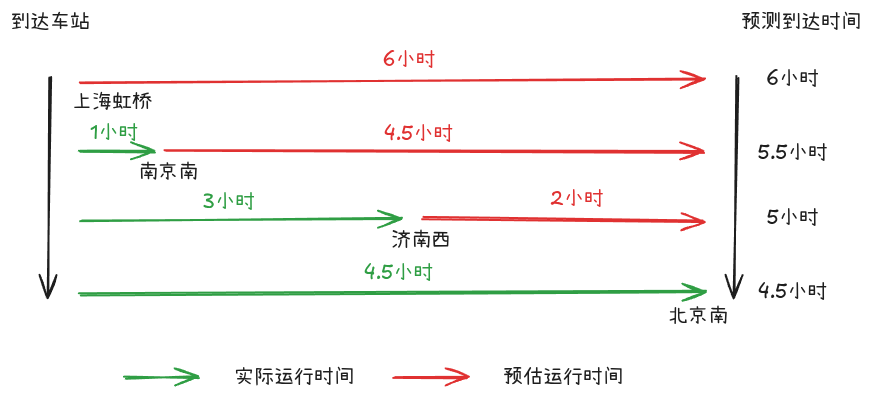
\includegraphics[width=0.5\linewidth]{../images/TD-learning-example.png}
        \caption{Illustration of TD learning}
        \label{fig:td_learning_intuition}
    \end{figure}
    也就是说，TD learning本质上是
    \begin{center}
        \textbf{通过新的信息和新的预测来更新旧的预测}。
    \end{center}
\end{frame}

\begin{frame}{Temporal Difference Learning}
    Temporal difference (TD) learning 通过相邻两步的转换关系来近似value function。注意到，
    \begin{equation}
        V^\pi(s) =\mathbb{E}^\pi[r_0 + \gamma V^\pi(s_1)\mid s_0=s]
    \end{equation}

    我们将

    \begin{equation}
        \overline{V}_t = r_t + \gamma V^\pi(s_{t+1})
    \end{equation}
    称为 TD target. 将
    \begin{equation}
        \delta_t = V^\pi(s_t) - \left(r_t + \gamma V^\pi(s_{t+1})\right)
    \end{equation}
    称为 TD error. 

\end{frame}

\begin{frame}{Temporal Difference Learning}
    当 $\mathcal{S}$ 比较大或者连续时，我们构造损失函数
    \begin{equation}
    \min_{\phi} \mathcal{L}(\phi) =\mathbb{E}\left[\frac12\left(V_\phi(s)-V^\pi(s)\right)^2\right]=\mathbb{E}\left[\left(V_\phi(s)- r_0-\gamma V^\pi(s_1)\right)^2\right]
    \end{equation}
    对应的梯度为
    \begin{equation}
    \nabla_\phi \mathcal{L}(\phi) =\mathbb{E}\left[\left(V_\phi(s)- r_0-\gamma \boxed{V^\pi(s_1)}\right)\nabla_\phi V_\phi(s)\mid s_0=s\right]
    \end{equation}
    令
    \begin{equation}
    g := \left(V_\phi(s)- r_0-\gamma \boxed{V^\pi(s_1)}\right)\nabla_\phi V_\phi(s)
    \end{equation}
    但是，这里存在的问题在于，我们使用了 $V^\pi(s_1)$, 而这个值是未知的，因此，一个做法是使用当前的 value function $V_\phi$ 来进行代替，即
    \begin{equation}
    \nabla_\phi \mathcal{L}(\phi) \approx \mathbb{E}\left[\left(V_\phi(s)- r_0-\gamma V_\phi(s_1)\right)\nabla_\phi V_\phi(s)\mid s_0=s\right]
    \end{equation}
\end{frame}

\begin{frame}{Temporal Difference Learning--Naive version}
    这样，我们结合 TD 和 GSD 的算法就变成了

    \begin{algorithm}[H]
        \caption{Value function approximation with TD (not correct)}
        \While{not converged}{
            $s_0\sim p_0$, $a_0\sim\pi(\cdot\mid s_0)$, $(r_0,s_1)\sim p(\cdot, \cdot\mid s_0,a_0)$\;
            
            $y = \begin{cases}
                    r_0 + \gamma V_\phi(s_1), & \text{if } s_1 \neq \text{<term>} \\
                    r_0,                      & \text{otherwise}
                \end{cases}$\;
            
            $g = (V_{\phi}(s_0) - y) \nabla_\phi V_{\phi}(s_0)$\;
            
            update $\phi$ using $g$ with an optimizer\;
        }
    \end{algorithm}
\end{frame}

\begin{frame}[fragile]{Temporal Difference Learning--Analysis}
    接下来，我们需要关注如何计算 $g$,  直接通过 $g=\left(V_\phi(s)- r_0-\gamma V_\phi(s_1)\right)\nabla_\phi V_\phi(s)$ 来进行计算，这在数学上是没有问题的，但是从自动微分的角度不对，比如 Pytorch 对应的实现应该是

    \begin{lstlisting}[language=python]
    pred = V_phi(s0)
    target = r + gamma * V_phi(s1)
    td_error = pred - target    
    loss = 0.5 * td_error ** 2
    loss.backward()
    \end{lstlisting}
    
    可以看到，我们实际上求的梯度是
    \begin{equation}
        \nabla_\phi\left[\frac12\left(V_\phi(s)-(r+\gamma V_\phi(s'))\right)^2\right]=(V_\phi(s)-(r+\gamma V_\phi(s'))(\nabla_\phi V_\phi(s)-\nabla_\phi V_\phi(s'))
    \end{equation}
    
    这显然与 $g$ 不相等
\end{frame}

\begin{frame}[fragile]{Temporal Difference Learning--Analysis}
    \small
    为了解决这个问题，我们需要使用 stop-gradient 的技巧来避免 $V_\phi(s')$ 参与反向传播，这个时候，我们的目标函数就变成了
    \begin{equation}
    \frac12\left(V_\phi(s)-(r+\gamma\ \mathrm{sg}[V_\phi(s')])\right)^2
    \end{equation}
    其中 $\mathrm{sg}[\cdot]$ 是 stop-gradient operator, 满足
    \begin{equation}
    \mathrm{sg}[x] = \begin{cases}
    x &\text{forward pass}\\
    0 &\text{backward pass}
    \end{cases}
    \end{equation}
    这样其梯度就是
    \begin{equation}
    \nabla_\phi\left[\frac12\left(V_\phi(s)-(r+\gamma\ \mathrm{sg}[V_\phi(s')])\right)^2\right]=(V_\phi(s)-(r+\gamma V_\phi(s'))\nabla_\phi V_\phi(s)=g
    \end{equation}
    对应的 python 代码为
    \begin{lstlisting}[language=python]
    pred = V_phi(s0)
    target = r + gamma * V_phi(s1)
    td_error = pred - target.detach()  # stop gradient operator
    loss = 0.5 * td_error ** 2
    loss.backward()
    \end{lstlisting}
\end{frame}

\begin{frame}{Temporal Difference Learning--Algorithm}
    最终，我们得到了一个简单的 TD 算法，其伪代码为
    \begin{algorithm}[H]
        \caption{Value function approximation with TD}
        \While{not converged}{
            $s_0 \sim p_0$, $a_0 \sim \pi(\cdot \mid s_0)$, $(r_0, s_1) \sim p(\cdot, \cdot \mid s_0, a_0)$\;
            
            $y = \begin{cases}
                    r_0 + \gamma \, \mathrm{sg}[V_\phi(s_1)], & \text{if } s_1 \neq \text{<term>} \\
                    r_0,                                      & \text{otherwise}
                \end{cases}$\;
            
            $g = (V_{\phi}(s_0) - y) \nabla_\phi V_{\phi}(s_0)$\;
            
            update $\phi$ using $g$ with an optimizer\;
        }
    \end{algorithm}
    \begin{block}{Remark}
        上述这种做法其实是 semi-gradient methods, 这类方法在参数更新时，只计算部分梯度。
        虽然这种方法牺牲了严格的梯度下降性质，但是其能够保证更好的表现。
    \end{block}
\end{frame}

\begin{frame}{k-step TD learning}
    我们可以进一步推广 TD 到多步的场景，注意到
    \begin{align}
    V^\pi(s) &=\mathbb{E}^\pi[r_0 + \gamma V^\pi(s_1)\mid s_0=s]\\
    &=\mathbb{E}^\pi[r_0 + \gamma \mathbb{E}^\pi[r_1 + \gamma V^\pi(s_1)\mid s_1]\mid s_0=s]\\
    &= \mathbb{E}^\pi[\mathbb{E}^\pi[r_0 + \gamma r_1 + \gamma^2 V^\pi(s_2) \mid s_1] \mid s_0=s] 
    \end{align}
    由重期望定理 (Law of Total Expectation, see Appendix Frame~\ref{law-of-total-expectation})
    \begin{equation}
    \mathbb{E}^\pi[\mathbb{E}^\pi[X \mid s_1] \mid s_0=s] = \mathbb{E}^\pi[X \mid s_0=s]
    \end{equation}
    因此：
    \begin{equation}
    V^\pi(s) = \mathbb{E}^\pi[r_0 + \gamma r_1 + \gamma^2 V^\pi(s_2) \mid s_0=s]
    \end{equation}
    重复这个过程 k 次,得到 k 步展开：
    \begin{equation} 
        V^\pi(s) = \mathbb{E}^\pi\left[\sum_{i=0}^{k-1} \gamma^i r_i + \gamma^k V^\pi(s_k) \mid s_0=s\right]
    \end{equation}
\end{frame}

\section{Reinforcement Learning: Value based methods}


\section{Reinforcement Learning: Policy based methods}


\section{Reinforcement Learning: Actor-Critic methods}


\section{RL for LLM: TRPO and PPO}

\section{RL for LLM: DPO}


\section{RL for LLM: GRPO}


% ===========================================================================
\section{References}
% ===========================================================================


\begin{frame}[allowframebreaks]
    \frametitle{References}
    \bibliographystyle{amsalpha}
    \bibliography{reference.bib}
\end{frame}

% \begin{frame}{References}
%   \footnotesize
%   \begin{itemize}
%     \item \href{https://blog.eleuther.ai/transformer-math/}{transformer-math} (EleutherAI)
%     \item \href{https://kipp.ly/transformer-inference-arithmetic/}{transformer inference arithmetic}
%     \item Reducing Activation Recomputation in Large Transformer Models (arXiv:2205.05198)
%     \item A Survey on Large Language Model Acceleration based on KV Cache Management (arXiv:2412.19442)
%     \item Efficient Large Language Models: A Survey (arXiv:2312.03863)
%     \item \href{https://maosong.website/p/notes-on-adamw/}{notes on AdamW}, \href{https://maosong.website/p/notes-on-flashattention/}{notes on Flash Attention}
%   \end{itemize}
% \end{frame}


\appendix

\begin{frame}[label=law-of-total-expectation]{Law of Total Expectation}
    TODO
\end{frame}

\begin{frame}[label=fixed-point-theorem]{Fixed Point Theorem*}
    \begin{block}{Fixed Point Theorem}
        给定函数 $f:\mathbb{R}^n\to\mathbb{R}^n$, 如果 $f$ 是一个 contraction mapping, 则 $f$ 具有如下性质
        \begin{enumerate}
            \item Existence: 存在 fixed point $x^*\in\mathbb{R}^n$ 满足 $f(x^*)=x^*$.
            \item Uniqueness: fixed point $x^*$ 唯一。
            \item Algorithm: 对任意 $x^0\in\mathbb{R}^n$, 使用迭代算法 $x_{k+1}=f(x_k)$ 产生的序列 $\{x_k\}_{k=0}^{\infty}$ 收敛到 fixed point $x*$, 且收敛速度为指数级。
        \end{enumerate}
    \end{block}
\end{frame}

\begin{frame}{Fixed Point Theorem--Cauchy Sequence}
    \begin{block}{Cauchy Sequence}
        一个序列 $\{x_k\}_{k=0}^{\infty}$ 被称为柯西列 (Cauchy sequence) 当且仅当对任意 $\epsilon>0$, 都存在 $N>0$, 使得
        \begin{equation}
            \|x_m-x_n\| <\epsilon,\forall m, n>N
        \end{equation}
    \end{block}

    \begin{theorem}
        一个序列 $\{x_k\}_{k=0}^{\infty}$ 是收敛列当且仅当它是柯西列。
    \end{theorem}
\end{frame}

\begin{frame}{Fixed Point Theorem--Proof}
    \begin{proof}
        我们首先证明由 $x_k=f(x_{k=1})$ 产生的序列 $\{x_k\}_{k=1}^{\infty}$ 是收敛的。
        注意到 $f$ 是一个 contraction mapping, 因此
        \begin{equation}
            \|x_{k+1}-x_k\| = \|f(x_k)-f(x_{k-1})\|\leq \gamma \|x_k-x_{k-1}\|
        \end{equation}
        迭代下去，我们就得到
        \begin{equation}
            \|x_{k+1}-x_k\|\leq \gamma \|x_k-x_{k-1}\|\leq\cdots\leq \gamma^k \|x_1-x_{0}\|
        \end{equation}
        现在我们证明序列 $\{x_k\}_{k=1}^{\infty}$ 是一个柯西列：
        \begin{equation}
        \begin{aligned}
        \|x_m-x_n\| &= \|x_m-x_{m-1}+x_{m-1}-\cdots-x_{n+1}+x_{n+1}-x_n\|\\
        &\leq \sum_{i=n}^{m-1}\|x_{i+1}-x_i\|\leq \sum_{i=n}^{m-1}\gamma^i \|x_{1}-x_0\|\leq \frac{\gamma^n}{1-\gamma}\|x_{1}-x_0\|.
        \end{aligned}
        \end{equation}
        从而，序列 $\{x_k\}_{k=1}^{\infty}$ 是一个柯西列, 因此也是一个收敛列。
    \end{proof}
\end{frame}

\begin{frame}{Fixed Point Theorem--Proof}
    \begin{proof}
        接下来，我们证明 $x^*=\lim_{k\to\infty}x_k$ 是 $f(x)$ 的不动点，注意到
        \begin{equation}
            \|f(x_k)-x_k\| = \|x_{k+1}-x_k\|\leq \gamma^k\|x_1-x_0\| \to 0, k\to\infty
        \end{equation}
        我们有 $\lim_{k\to\infty}f(x_k)=\lim_{k\to\infty}x_k$ , 由于 contraction mapping 一定是连续的，因此我们就可以得到 $f(x^*)=x^*$.
        然后，我们证明不动点唯一。假设还存在一个另外一个不动点 $x'\neq x^*$ 满足 $f(x')=x'$, 那么
        \begin{equation}
            \|x'-x^*\| = \|f(x')-f(x')\| \leq \gamma \|x'-x^*\|
        \end{equation}
        由于 $\gamma\in(0,1)$, 因此上述等式当且仅当 $\|x'-x^*\|=0$, 这与前面假设矛盾，因而不动点是唯一的。
    \end{proof}
\end{frame}

\begin{frame}{Fixed Point Theorem--Proof}
    \begin{proof}
        最后，我们证明 $x_{k+1}=f(x_k)$ 这个算法的收敛速度为指数级，注意到
        \begin{equation}
            \|x^*-x_n\| = \lim_{m\to\infty}\|x_m-x_n\| \leq \frac{\gamma^n}{1-\gamma}\|x_1-x_0\|
        \end{equation}
        因为 $\gamma <1$, 因此收敛速度为指数级。
    \end{proof}
\end{frame}

\end{document}
